\section{Feature detection}  \label{sec:features}

\begin{figure}[t]
    \centering
    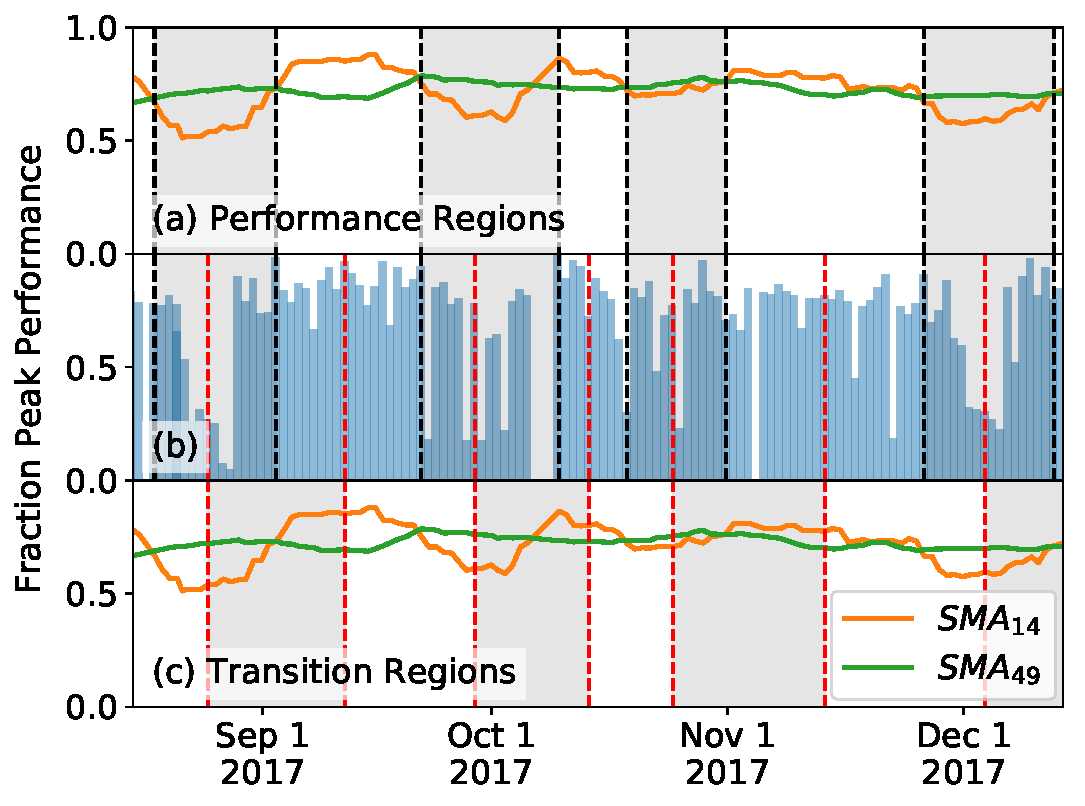
\includegraphics[width=1.0\columnwidth]{segment-explain}
    \vspace{-.35in}
    \caption{Example of overlaying two simple moving averages (SMAs) to identify (a) \emph{performance regions} and (c) \emph{transition regions} in the Edison scratch2 IOR/fpp write dataset.  Middle pane (b) includes raw performance measurements (blue bars) with both SMA crossovers (black dashed lines) and performance region centroids (red dashed lines).}
    \label{fig:segment-explain}
%   \vspace{-.3in}
% UP01 to UP03 upgrade, UP03 to UP04
\end{figure}

The data in Figure \ref{fig:summary-heatmap} demonstrates that nominally optimal I/O performance for a given system evolves over time.
As a result, it is often not meaningful to express the performance of an application as being good or bad with respect to an absolute peak performance;
rather, "bad" performance (and its causes) should be classified with respect to what qualifies as "good" performance for a timescale of interest.
To address this issue, we propose applying simple moving averages (SMAs) as a means to identify correlated performance trends in production parallel file systems.
This approach has commonly been applied in the context of financial market technical analysis, where moving averages are used to attenuate the day-to-day volatility in the price movements of underlying assets and to help identify larger trends in these movements~\cite{}.

Given a time window of width $w$, we define the SMA for a metric $M$ at time $t$ as the average value of $M$ over ${-0.5w <= t < +0.5w}$;
when chosen to be sufficiently wide (e.g., $w = 49$ days), the resulting $\textup{SMA}_{49}$ provides a rapid visual means to identify performance degradation or recovery that lasts for $O(\textup{weeks})$.  Superimposing a second SMA with a shorter window, such as $\textup{SMA}_{14}$, then allows us to distinguish short-term performance anomalies that last for $O(\textup{days})$ from longer-term performance evolution.

In the following analysis, we apply this SMA-based approach to procedurally identify and classify performance variation at all time scales, ranging from long-term system health issues to transient performance loss due to probabilistic contention.
We define $\textup{SMA}_{long}$ and $\textup{SMA}_{short}$ as simple moving averages and adjust $w_{short}$ and $w_{long}$ to reflect the sensitivity to performance transients and long-term performance evolution, respectively.
The exact choice of $w_{short}$ and $w_{long}$ are somewhat arbitrary; empirically, adjusting these values by $\pm 5 \%$ was not found to cause substantive changes to the results.

% J_{app, rw, sys}
We then partition a set of performance observations $J_{app, rw, sys}$ into \emph{performance regions}, which are non-overlapping subsets of $J_{app, rw, sys}$ that are bounded by the intersection between $\textup{SMA}_{long}$ and $\textup{SMA}_{short}$.
Figure \ref{fig:segment-explain}a illustrates this partitioning of the IOR/fpp write workload measurements on Edison's scratch2 file system;
dashed lines represent the intersection of $\textup{SMA}_{long}$ and $\textup{SMA}_{short}$, and performance regions are shaded in alternating gray and white.
As Figure \ref{fig:segment-explain}a illustrates, using SMA crossovers to identify performance regions results in temporally contiguous subsets of performance measurements that capture a period of time with consistently good (${\textup{SMA}_{short} > \textup{SMA}_{long}}$) or bad (${\textup{SMA}_{short} < \textup{SMA}_{long}}$) performance.

To understand the causes of the \emph{transitions} between performance regions, we also partition $J_{app, rw, sys}$ into \emph{transition regions}.
For each performance region, we identify the temporally center-most observation as the centroid of that performance region, as illustrated in Figure \ref{fig:segment-explain}b, as red dashed lines.
We then define transition regions as those regions bounded by centroids (Figure \ref{fig:segment-explain}c), and each transition region overlaps with exactly two performance regions and vice versa.
The principal difference between the two is that performance regions contain observations that are uniformly good or uniformly bad, and transition regions capture performance transitioning from bad to good or vice versa.

